\section{Introduction}
\label{sec:intro}

\subsection{Basic Structure of VAE}

VAE consists of three main components: the encoder, the latent space, and the decoder ~\cite{chan2025tutorial}.

\begin{itemize}
    \item \textbf{Encoder:}
    The encoder takes input data and transforms it into a representation within the \textit{latent space}. Unlike traditional AE, the encoder in VAE learns a probabilistic distribution instead of fixed points, allowing for more flexible and uncertainty-aware data representation.

    \item \textbf{Latent Space:}  
    The latent space in VAE is a continuous and well-organized space. Each point in this space represents a latent state of the data. The continuity and smoothness of the latent space allow the model to generate new data by sampling points from it.

    \item \textbf{Decoder:}  
    The decoder receives information from the latent space and reconstructs the original data. Additionally, it can generate new data by sampling points from the latent space, making VAE a highly effective generative model.
\end{itemize}

The key strength of VAE lies in its ability to balance accurate data reconstruction with the organization of the latent space, facilitating meaningful data generation.

\begin{figure}[H]
    \centering
    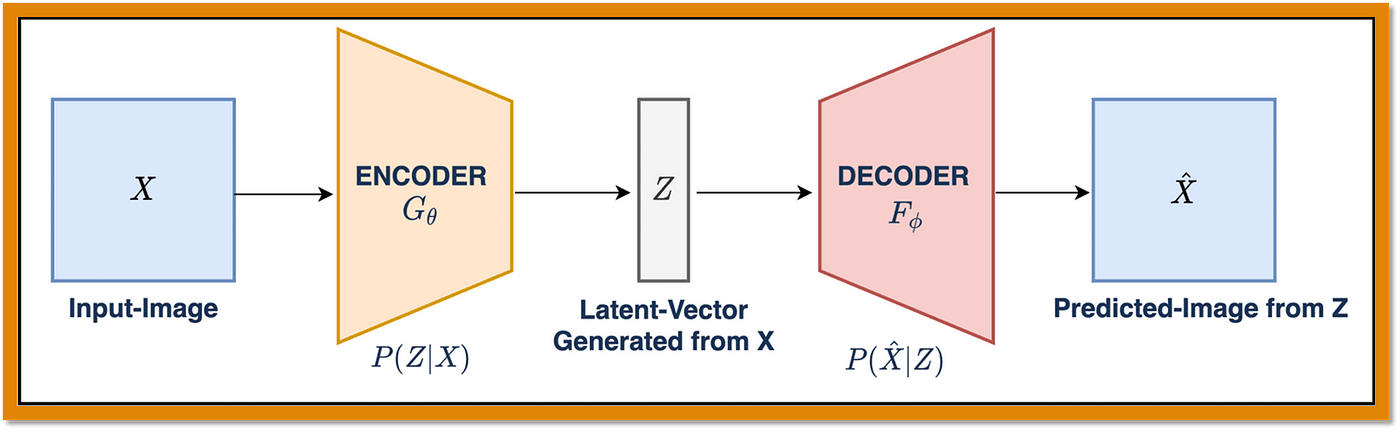
\includegraphics[width=1.0\linewidth]{sec/VAE.png}
    \caption{VAE Structure}
\end{figure}

\subsection{Why Choose VAE}

While the traditional Autoencoder excels at compressing and reconstructing data, it has limitations that VAE addresses. Here are the main reasons why VAE is preferred:

\begin{itemize}
    \item \textbf{Data Generation:}  
    Traditional AE only reconstructs learned data, whereas VAE can generate new data by sampling from the latent space.

    \item \textbf{Smooth Latent Space:}  
    The latent space of VAE is continuous and smooth, ensuring that generated samples are reasonable even when sampled randomly.

    \item \textbf{Better Generalization:}  
    VAE utilizes regularization techniques to avoid overfitting and improve its generalization capabilities on unseen data.

    \item \textbf{Uncertainty Handling:}  
    VAE can learn and represent uncertainty in the data, a capability absent in traditional AE.
\end{itemize}

Thanks to these advantages, VAE serves as a powerful tool for data compression, reconstruction, and diverse applications such as image synthesis, anomaly detection, and data augmentation.